\documentclass[12pt]{article}
\usepackage{amsmath, amssymb, amsthm}
\usepackage{graphicx}
\usepackage{hyperref}
\usepackage{float}
\usepackage{geometry}
\geometry{margin=1in}

\title{CS461 Homework 2}
\author{Mannan Shukla}
\date{Due: October 20, 2024}

\begin{document}

\maketitle

\section*{Problem 1: Linear Models and MMSE Regression}

\subsection*{1.1 Data Matrix}
Write out the data matrix \( \Phi \) based on the given data points.

\[
\Phi = \begin{bmatrix}
1 & x_{11} & x_{12} & x_{13} \\
1 & x_{21} & x_{22} & x_{23} \\
1 & x_{31} & x_{32} & x_{33} \\
1 & x_{41} & x_{42} & x_{43} \\
\end{bmatrix}
\]

\subsection*{1.2 Exact or MMSE Solution}
Discuss whether the normal equation will give an exact solution or an MMSE approximated solution.

\subsection*{1.3 Solving the Normal Equation}
Explain the invertibility of \( \Phi^T \Phi \). Provide your solution for \( \mathbf{w} \).

\subsection*{1.4 Comparing the Models}
Compare the original model \( y = 1 + 2x_1 + 3x_2 + 4x_3 \) with your solution and discuss the differences.

\subsection*{1.5 Adding New Data Points}
Add the new data points and solve for \( \mathbf{w} \). Discuss the chance of obtaining the original model.

\subsection*{1.6 Column Removal for Unique Solution}
Examine the data matrix and identify which column to remove to ensure a unique solution.

\section*{Problem 2: Lagrangian Function and KKT Conditions}

\subsection*{2.1 MMSE Objective Function}
Define the MMSE objective function \( J(\mathbf{w}) \) and solve for the optimal solution \( (w_0, w_1) \).

\subsection*{2.2 Lagrangian Function}
Define the Lagrangian function for the constrained optimization problem.

\subsection*{2.3 Solving for \( \lambda \) and \( \mathbf{w}^* \)}
Based on KKT conditions, compute the optimal Lagrangian parameter \( \lambda \) and \( \mathbf{w}^* \) for \( C = \{0.5, 1, 2, 3\} \).

\section*{Problem 3: Learning Sinusoidal Functions}

\subsection*{3.1 Implementing Ordinary MMSE Regression}
Describe your code implementation in `ols\_regression.py` for the MMSE regression model. Report the average validation error across five cross-validations.

\subsection*{3.2 Ridge Regression}
Describe your code implementation in `ridge\_regression.py` for the ridge regression model. Plot the averaged validation error for different values of \( \lambda \).

\begin{figure}[H]
    \centering
    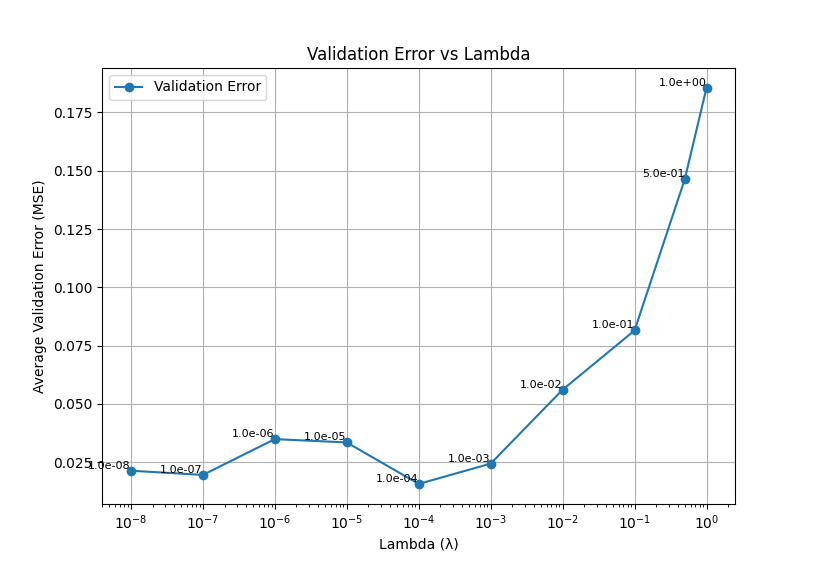
\includegraphics[width=0.7\textwidth]{ridge_regression_plot.png}
    \caption{Validation Error vs. \( \lambda \)}
\end{figure}

\subsection*{3.3 Plot the Models}
Plot the models \( w(\lambda = 0) \) and \( w(\lambda^*) \) over the range \( 0 \leq x \leq 1 \).

\subsection*{3.4 Evaluate with Test Data}
Evaluate both models on the test dataset and report the test MSE for each.

\subsection*{3.5 Larger Dataset}
Explain the regression model you implemented in `ols\_regression\_largeset.py` and plot the model over the range \( 0 \leq x \leq 1 \).

\subsection*{3.6 Controlling Effective Complexity}
Propose two solutions to control the effective complexity in machine learning.

\section*{Problem 4: Eigenface and Spectral Decomposition}

\subsection*{4.1 Covariance Matrix and Spectral Decomposition}
Compute the covariance matrix \( \text{COV}(X, X) \) and its eigenvalue decomposition.

\subsection*{4.2 Approximating the Test Image}
Approximate the test image using different \( M \) values (2, 10, 100, 1,000, 4,000). Present the corresponding images in your report.

\begin{figure}[H]
    \centering
    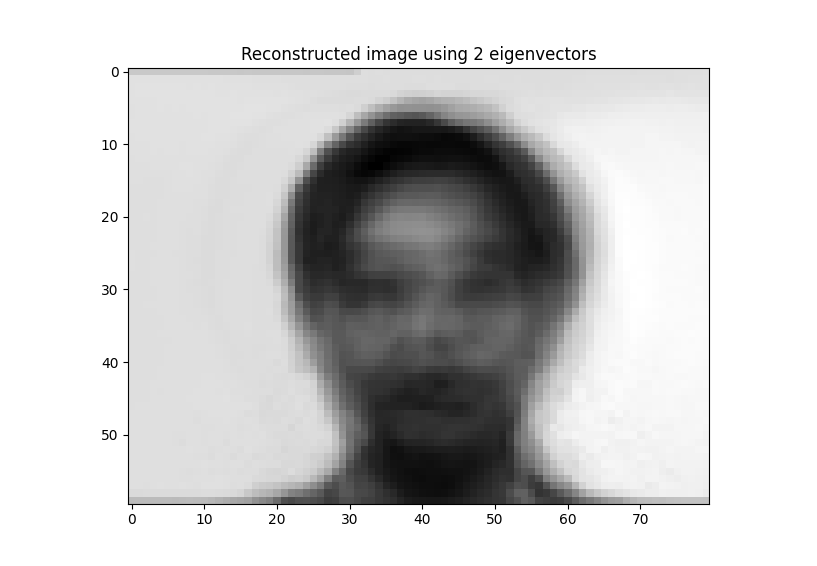
\includegraphics[width=0.3\textwidth]{eigenface_M2.png}
    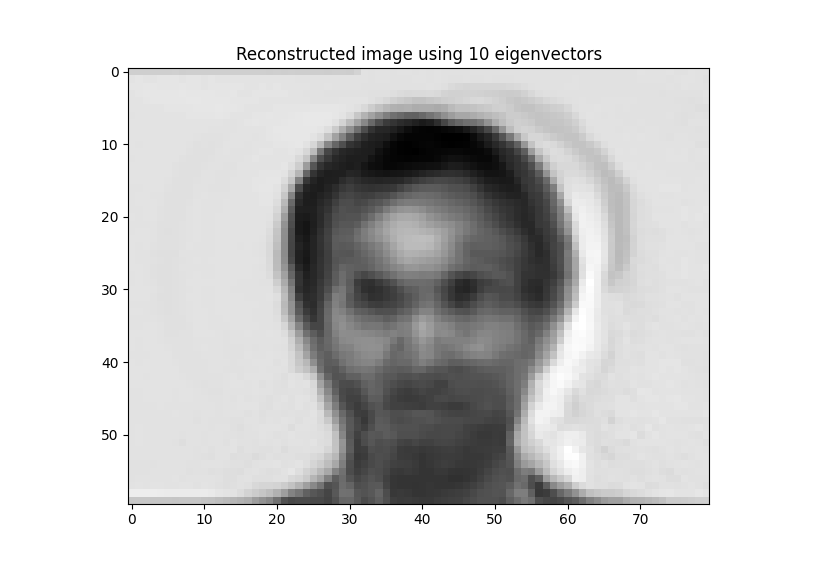
\includegraphics[width=0.3\textwidth]{eigenface_M10.png}
    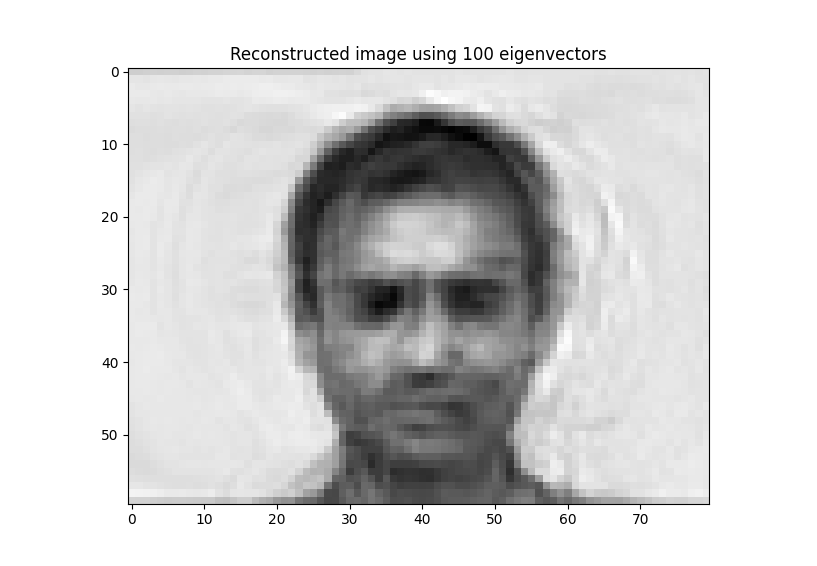
\includegraphics[width=0.3\textwidth]{eigenface_M100.png}
    \caption{Approximations with different M values}
\end{figure}

\subsection*{4.3 Eigenvectors for the Largest Eigenvalues}
Show the grayscale images of the eigenvectors corresponding to the ten largest eigenvalues and explain how they capture facial features.

\section*{Problem 5: Extra Points - Year of Made Prediction}

\subsection*{5.1 Dimensional Reduction and Whitening}
Reproduce the scatter plots for \( M = 1 \) and \( M = 2 \). Discuss why the 2-D projection is more promising for year prediction.

\subsection*{5.2 Training the Model}
Explain your implementation in `year\_train.py` and describe how you selected the polynomial basis and validated the model.

\subsection*{5.3 Testing the Model}
Report the test MSE and identify the most and least accurate predictions.

\end{document}
